\documentclass[12pt]{article}  % [12pt] option for the benefit of aging markers

% amssymb package contains more mathematical symbols
\usepackage{amssymb,amsthm}

% graphicx package enables you to paste in graphics
\usepackage{graphicx}
\usepackage{auto-pst-pdf}

% embed source inside latex
\usepackage[procnames]{listings}
\usepackage{color}

% ALGORITHM
\usepackage{algorithm}
\usepackage{algpseudocode}
\usepackage{hyperref}
\usepackage{booktabs}
\usepackage{enumitem}

%%%%%%%%%%%%%%%%%%%%%%%%%%%%%%%%%
%
%    Page size commands.  Don't worry about these
%
\setlength{\textheight}{220mm}
\setlength{\topmargin}{-10mm}
\setlength{\textwidth}{150mm}
\setlength{\oddsidemargin}{0mm}

%%%%%%%%%%%%%%%%%%%%%%%%%%%%%%%%%%%%%%%%%%%%%%%%%%%%%%%%%%%%%%%
%
%    Definitions of environments for theorems etc.
%
\newtheorem{theorem}{Theorem}[section]          % Theorems numbered within sections - eg Theorem 2.1 in Section 2.
\newtheorem{corollary}[theorem]{Corollary}      % Corollaries etc. will be counted as Theorems for numbering
\newtheorem{lemma}[theorem]{Lemma}              % eg Lemma 3.1, ... Theorem 3.2, ... Corollary 3.3.
\newtheorem{proposition}[theorem]{Proposition}
\newtheorem{conjecture}[theorem]{Conjecture}

\theoremstyle{definition}
\newtheorem{definition}[theorem]{Definition}

\theoremstyle{remark}
\newtheorem{remark}[theorem]{Remark}
\newtheorem{example}[theorem]{Example} 

%%%%%%%%%%%%%%%%%%%%%%%%%%%%%%%%%%%%%%%%%%%%%%%
%
%        Preamble material specific to your essay
%
\title{Simulation of M/M/2/2+5 Queueing System}
\author{Jiaqi Yan, Ping Liu\\
CS555 Project\\
supervised by
Edward Chlebus}

\begin{document}
\maketitle

% \newpage                     % optional page break
\begin{abstract}
In this project, we simulate and analyze the M/M/2/2+5 queueing system. 
To generate generate packet arriving time and processing time, we use Python's built-in \textit{random} module, which is validated carefully.
Then we apply the \textbf{Welch graphical procedure} to eliminate the warm-up period in the simulation.
With the stationary region, we then analyze the system's properties such as blocking probability and mean number of packet in the system.
The 90\% confidence interval for these properties are also given.
\end{abstract}

% optional page break
\newpage
\tableofcontents

% optional page break
\newpage
\section{Discrete Event Simulation}\label{sec:des}
We designed and implemented our own simple simulator for M/M/2/2+5 queueing system. The simulation workflow is shown in Algorithm \ref{alg:simulator}.
The while loop will keep consume event in the $event\_list$ until we handled all the packets.
Whenever there is unseen packets, we create an arrival event and insert it to the list.
This list thus should be maintained in order with respect to events' time stamp, which is determined as soon as we create a \texttt{event} object.
Also based on this time stamp, we will pop up the next event we should handle from the list according to the event type, either $arrival$ or $departure$.

If the type is $departure$, we first check number of arrived but waiting packets in the system.
When no packets need to be served at this moment, set the server this packet is leaving from to $idle$;
otherwise, just decrease this $waiting$ counter.
Anyway, we just served a packet.
This means the counter for served packet should increase.
We can also calculate the entire time this packet is in the system, from it entering until its exit, e.g. current clock.

For $arrival$ event, 
\begin{algorithm*}[t]
\caption{Core of Discrete Event Simulation}
\label{alg:simulator}
\begin{algorithmic}[1]
\Function{simulation\_core}{$arrive\_time\_seq$, $serve\_time\_seq$}
\State{let $arrive\_time\_seq$ denote the arriving time of each packet}
\State{let $serve\_time\_seq$ denote the service time of each packet}
\State{let $N$ denote the number of total packets}
\While{$pkt\_served + pkt\_dropped < N$}
    \If{$pkt\_seen < N$}\Comment{Insert new arrival event to event list}
        \State $ts \gets arrive\_time\_seq[pkt\_seen]$
        \State{Create new arrival event $evt$ with time stamp $ts$ and id $pkt\_seen$}
        \State{Insert $evt$ to $event\_list$}
    \EndIf
    \State{Sort $event\_list$ based on events' time stamp}
    \State{Pop up the next event $evt_x$ we need to handle in $event\_list$}
    \State{$clock \gets evt_x.time\_stamp$}
    \If{$evt_x$ is departure event}
        \If{queue buffer is empty}
            \State{Set the status of the server $evt_x$ is leaving to $idle$}
        \Else
            \State{$--waiting$}
        \EndIf
        \State{$++pkt\_served$}
        \State{$evt\_x.exit_time \gets clock$}
        \State{$spending\_time \gets evt\_x.exit\_time - evt\_x.enter\_time$}
        \State{Record the spending time of packet of event $evt_x$}
    \EndIf
    \If{$evt_x$ is arrival event}
        \If{queue buffer is full}
            \State{$++pkt\_dropped$}
        \Else
            \If{There is available server}
                \State $id \gets evt_x.pkt\_id$
                \State $ts \gets clock + serve\_time\_seq[id]$
                \State{Choose an available server $s$}
                \State{Mark $s$ as $busy$}
            \Else
            \State $(ts, s) \gets $\Call{schedule\_departure}{  }
            \State $++waiting$
            \EndIf
            \State{Create new departure event $evt$ with time stamp $ts$}
            \State{$evt.enter\_time \gets clock$}
            \State{$evt.depart\_srv \gets s$}
            \State{Insert $evt$ to $event\_list$}
        \EndIf
    \EndIf
\EndWhile
\EndFunction
\end{algorithmic}
\end{algorithm*}



%\begin{center}
%\begin{tabular}{|r|r|r|r|r|r|r|}        % 7 columns, each right-justified
%\hline                                  % horizontal line between rows
 %& $R_1$ & $R_2$ & $R_3$ & $R_4$ & $R_5$ & $R_6$ \\ % header row
%\hline
%$R_1$ &   & 3 &   &   &    & \\
%\hline
%$R_2$ & 4 &   & 6 &   &    & \\
%\hline
%$R_3$ &   &   &   & 7 &    & \\
%\hline
%$R_4$ &   &   &   &   & 11 & \\
%\hline
%$R_5$ &   &   &   &   &    & 9 \\
%\hline
%$R_6$ &   & 8 & 5 &   &    & \\
%\hline
%\end{tabular}
%\end{center}

\section{Random Generator}
\subsection{Validation}
In M/M/2/2+5 queueing system, the number of packet arriving in a fixed interval follows \textbf{Poisson Distribution} and the service time for each packet follows \textbf{Exponential Distribution}.
These input data is generated by \textit{Numpy}'s \textit{random} module. Before running the simulator, it is important to test the wellness of this random generator.

We evaluate Numpy's random generator in two ways. First we generate random values follows uniform distribution and then plot their histogram.
As shown in Figure \ref{fig:uniform}, the number of random values falling into each interval is close to each other.
This means that the generated values are very close to uniformly distributed.
Besides, we compare the normalized histogram to the `best fit' curve of both uniform distribution and normal distribution in Figure \ref{fig:uniform} and \ref{fig:normal}.
From both figures we can say that the random generator generated random values of user-specified distribution.


\begin{figure}
\centering
        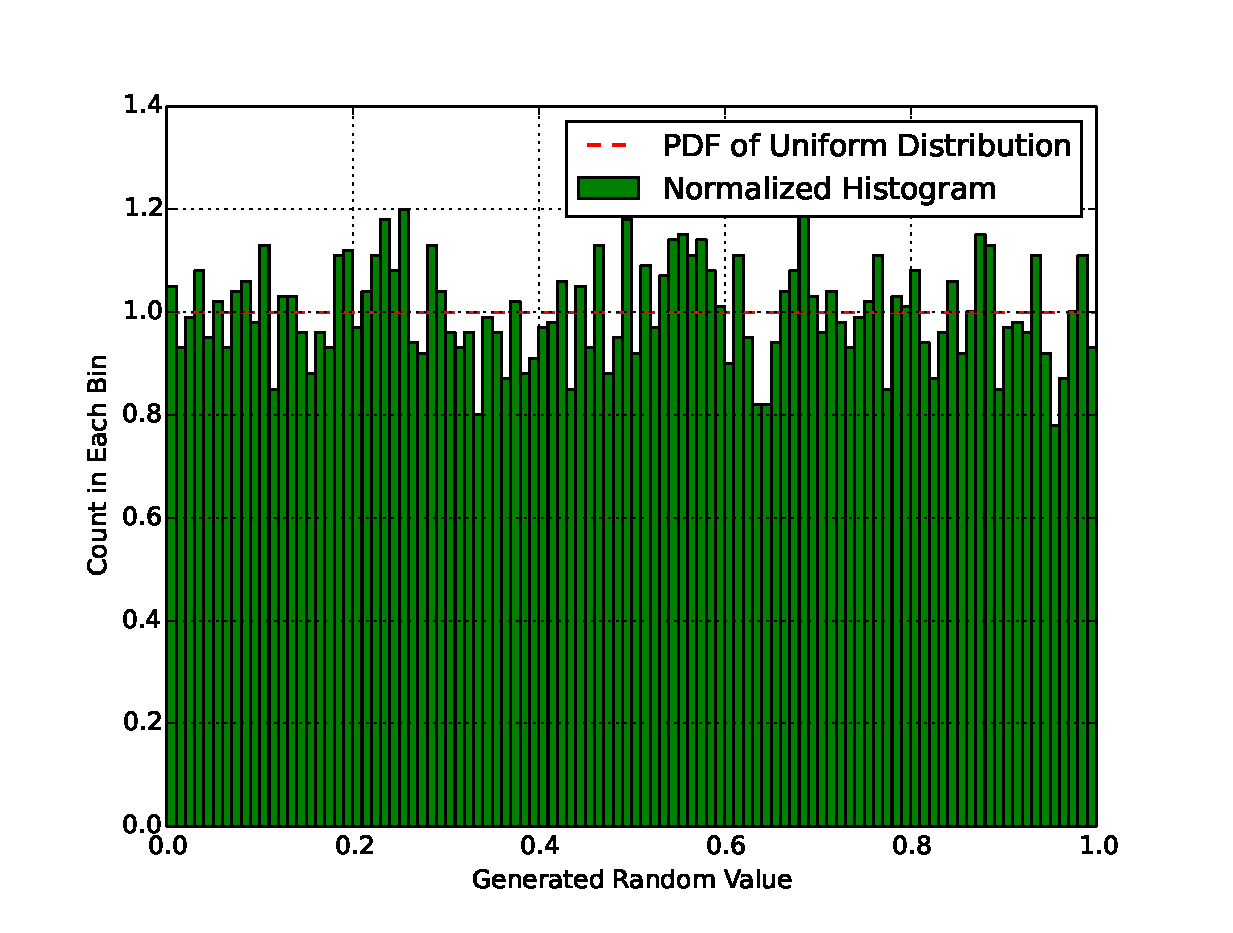
\includegraphics[scale=0.6]{rg_histogram.eps}
        \caption{Histogram of Uniform Random Values Generated by Numpy}
        \label{fig:uniform}
\end{figure}
\begin{figure}
        \centering
        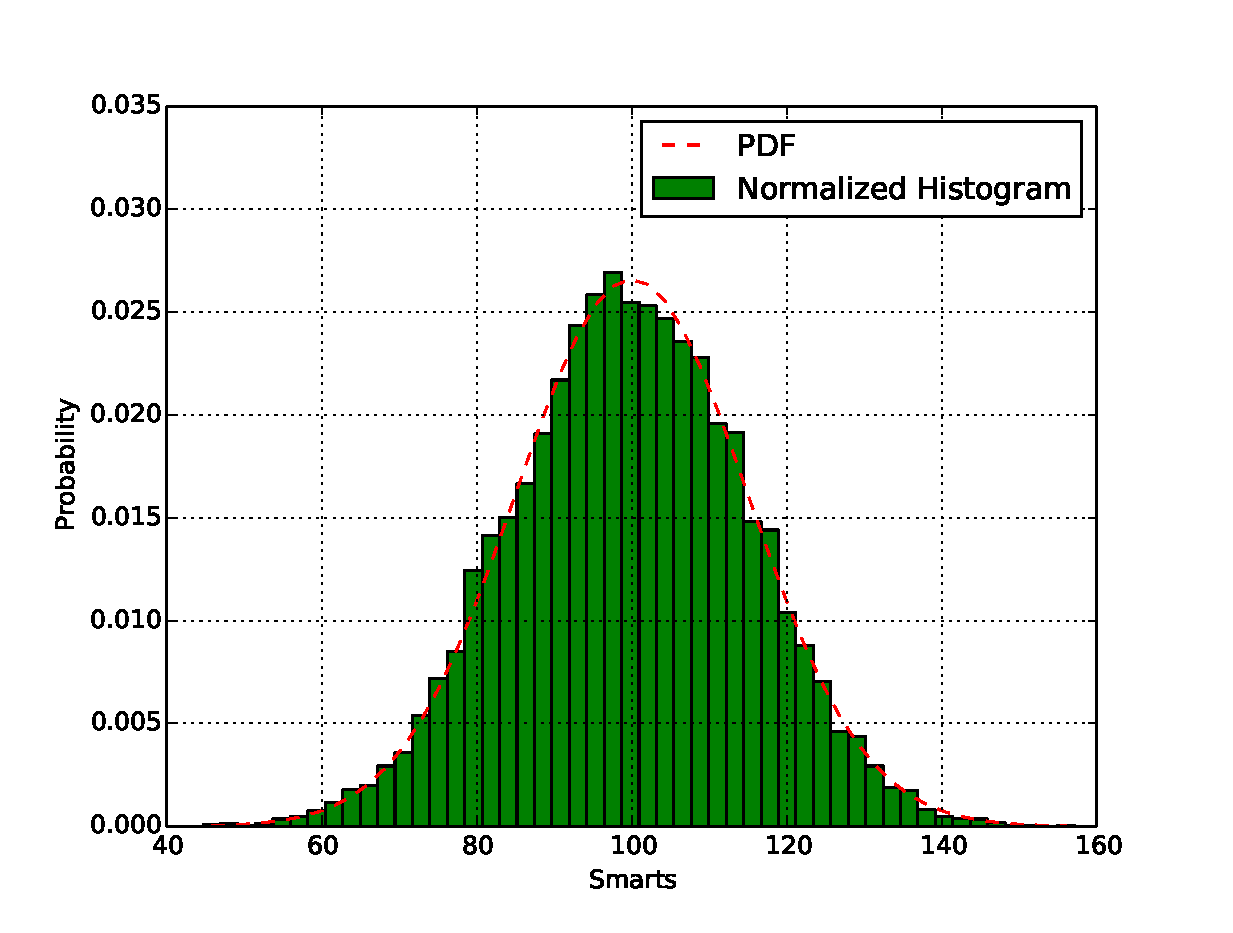
\includegraphics[scale=0.6]{rg_fitness.eps}
        \caption{Comparison to Best Fit Curve for Normal Distribution}
        \label{fig:normal}
\end{figure}

To generate different random value sequences, we feed the random generator a seed, which is the integral value of system current time.
That is the number of seconds since \textbf{Unix Epoch}.
We generated two sequences of 1000000 numbers each and use \textbf{t-test} to test statistically are they significantly different from each other.


\section{Eliminate Warm-up Period}



\section{System Properties at Stationary State}

\subsection{Blocking Probability}


\subsection{Mean Spending Time}


\subsection{Mean Number of Packet}





% Python code embedding configuration
%\definecolor{keywords}{RGB}{255,0,90}
%\definecolor{comments}{RGB}{0,0,113}
%\definecolor{red}{RGB}{160,0,0}
%\definecolor{green}{RGB}{0,150,0}
%\lstset{language=Python,
        %basicstyle=\ttfamily\small,
        %keywordstyle=\color{keywords},
        %commentstyle=\color{comments},
        %stringstyle=\color{red},
        %showstringspaces=false,
        %identifierstyle=\color{green},
        %procnamekeys={def,class,True},
        %frame=single,
        %numbers=left,
        %numbersep=5pt,
        %numberstyle=\tiny\color{blue},
        %rulecolor=\color{black},
        %caption={Simulation Discovery Process},
        %label=lst:while-loop,
        %language=Python,
%}
%\begin{lstlisting}
%while updated:
    %for r in routers:
        %for n in r.neighbors:
            %router_n = get_router_by_name(n, routers)
            %for n_name, n_row_col in router_n.topo.items():
                %n_msg = (n_name, n_row_col)
                %r.recv_msg(n_msg)
    %updated = False
    %for r in routers:
        %if r.update_topo_database():
            %updated = True
%\end{lstlisting}

%\begin{figure}[h]
%\centering
        %\includegraphics[width=0.8\textwidth, height=0.8\textheight]{progress.ps}
%\caption{Discovery Percentage as Function of Iteration for $R_1$ and $R_6$}
%\label{fig:progress}
%\end{figure}


%%%%%%%%%%%%%%%%%%%%%%%%%%%%%%%%%%%%%%%%%
%
%     Bibliography
%
%     Use an easy-to-remember tag for each entry - eg \bibitem{How97} for an article/book by Howie in 1997
%     To cite this publication in your text, write \cite{How97}.  To include more details such as
%     page, Chapter, Theorem numbers, use the form \cite[Theorem 6.3, page 42]{How97}.
%
%\begin{thebibliography}{99}

% 
% The usual convention for mathematical bibliographies is to list alphabetically
% by first-named author (then second, third  etc. author then date)
% websites with no author names should go by the site name
%


% Typical layout for reference to a journal article
%
%\bibitem{Bovey}
%J. D. Bovey, M. M. Dodson,                         % author(s)
%The Hausdorff dimension of systems of linear forms % article name
%{\em Acta Arithmetica}                             % journal name - italics
%{\bf 45}                                           % volume number - bold
%(1986), 337--358.                                   % (year), page range

%% Typical layout for reference to a book
%%
%\bibitem{Cassels}
%J. W. S. Cassels,                                  % author(s)
%{\em An Introduction to Diophantine Approximation},% title - italics
%Cambridge University Press, Cambridge, 1965.       % Publisher, place, date.

%% Typical layout for reference to a website
%%
%\bibitem{GAP}
%The GAP Group, GAP -- Groups, Algorithms, and Programming,  % Site name
%Version 4.5.6; 2012. % other information
%(http://www.gap-system.org)  % URL


%% Typical layout for reference to an online article
%%
%\bibitem{Howie}
%J. Howie,                                            % author(s)
%{\em Generalised triangle groups of type $(3,5,2)$}, % article name - italics
%http://arxiv.org/abs/1102.2073                       % URL
%(2011).                                              % (year)
%\end{thebibliography}

\end{document}
